
\documentclass{book}
%%%%%% General customization fetched from rahulbhadani.sty
\usepackage{bhadani_book}

%%%% Document specific customization goes here %%%%
\usepackage{fancyhdr}
 \renewcommand{\headrulewidth}{0pt}
\pagestyle{fancy}



\makeatletter
\newcommand{\globalcolor}[1]{%
  \color{#1}\global\let\default@color\current@color
}
\makeatother

\AtBeginDocument{\globalcolor{gray}}

\newcommand{\solution}{\textcolor{green}{\section{Solution:}}}
\newcommand{\intro}[1]{\textcolor{scarletred}{#1}}


% Custom Header and Footer
\fancyhf{}
\rhead{\textsc{Latex Book} -- \textsc{Page \thepage}}
\lfoot{\small{\textsc{Rahul Bhadani} -- \textsc{The University of Arizona}}}

%Document Title
\title{{ { \huge\textcolor{scarletred}{\textsf{Latex Book}}}}}
\author{\Large\textbf{Rahul Bhadani}\\ \textbf{\textsf{rahulbhadani@email.arizona.edu}}}

\makeindex  
\graphicspath{ {figures/} }
\begin{document}
%\fontsize{12}{16}\selectfont
\frontmatter
\maketitle
{{\sc \tableofcontents }}
%\listoffigures

\mainmatter
%%%%%%%%%%%%%%%% Question 1 %%%%%%%%%%%%%%%%%%%%%%%%
\chapter{First Chapter}
This is first chapter

\section{Some important questions}
It is  a section
\section{Some metrics }
Another section

\chapter{Second chapter}
\label{ch:01label}
Deep neural nets are learning intelligent behavior in a complex dynamic environment but there are cons: we have to train them. At the same time, trained agents can't do better than the training set. Solution: Use a policy-based approach and reward the agent whenever the agents do something good while penalizing them when agents do something undesirable. This is the principle behind the \textbf{Reinforcement Learning (RL)}. A general idea is depicted in \figref{fig:ch01RL}.

   \begin{figure}[htbp]
    \centering
        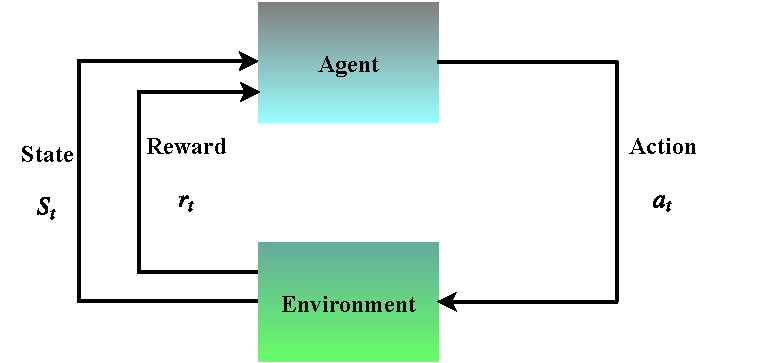
\includegraphics[trim={0.0cm 0.0cm 0.0cm 0.0cm},clip,width=0.75\linewidth]{RLdiagram.pdf}
    \caption{Reinforcement learning.}
    \label{fig:ch01RL}
    \end{figure}
    
\textbf{Policy network: }network in reinforcement learning to give output.
\begin{enumerate}
\item[--] Start with completely random network
\item[--] Produces random o/p.
\item[--] Feedback to (say) game engine
\item[--] loop continues
\item[--] Use scoreboard for reward/penalty
\item[--] Goal is to optimize the policy to receive as much reward as possible.
\end{enumerate}


\section{Terminology}

\chapter{Writing code in latex}
Install necessary packages:

\begin{minted}
[
framesep=2mm,
baselinestretch=1.2,
bgcolor=blue!30!white,
fontsize=\footnotesize,
]
{bash}
sudo apt-get install golang python3-dev python-dev libcupti-dev libjpeg-turbo8-dev \ 
make tmux htop chromium-browser git cmake zlib1g-dev libjpeg-dev  \
xvfb xorg-dev python-opengl libboost-all-dev libsdl2-dev swig
\end{minted}


\begin{mdframed}[linecolor=black, topline=true, bottomline=true,
  leftline=false, rightline=false, backgroundcolor=white!60!red]
    \inputminted[fontsize=\footnotesize, linenos, frame=lines]{matlab}{code/problem5.m}
\end{mdframed}

\bibliographystyle{IEEEtran}
\bibliography{IEEEabrv,bibliography}

\end{document}
